\upaper{0}{Предисловие}
\author{Божественный Советник}
\vs p000 0:1 В умах смертных Урантии\index{Урантия|textbf}\fnst{\textbf{Урантии} Синтетическое слово <<Ур\'антия>>, возможно, происходит от греческого \textgreek{οὐρανός} (небеса) и латинского суффикса \bibemph{-tia}, в комбинации придающих этому слову смысл <<наше место на небесах>>. Вообще, весь смысл этого Откровения в том, что он указывает каждому человеку на \bibemph{его место во Вселенной}.} --- таково название вашего мира --- существует огромная путаница относительно смысла таких терминов, как Бог, божественность и божество. Человеческие существа ещё больше озадачены и неуверенны относительно взаимосвязей божественных личностей, обозначаемых столь многочисленными названиями. Из\hyp{}за этой концептуальной бедности, связанной со столь большой путаницей в формировании идей, я был уполномочен сформулировать это вводное изложение для объяснения смыслов, которые должны быть присвоены определённым словесным символам, чтобы они могли быть использованы в дальнейшем в тех документах\fnst{\textbf{тех документах} Только документы 1--31 (т.е. Часть I) были составлены в рамках полномочий Орвонтонского корпуса. Данное Предисловие, как это станет ещё более ясно из следующих параграфов, относится только к этим документам, а не ко всему Откровению.}, которые Орвонтонский\fnst{\textbf{Орвонтонский}, Я произношу <<Орв\'онтонский>>.} корпус открывателей истины [truth revealers] был уполномочен перевести на английский\fnst{\textbf{английский} Причина, по которой Пятое Эпохальное Откровение <<дано>> на английском языке, проста: это родной язык доктора Уильяма С. Садлера, который достиг необходимой степени духовного и интеллектуального развития для работы в партнёрстве с Богом. Однако, во Вселенной всё взаимосвязано и целесообразно. Один из величайших духовных учителей <<русского пространства>> --- Лев Николаевич Толстой (1828--1910) --- уже изложил в достаточно полной и точной форме <<евангелие братства>>. Его полное собрание сочинений в 90 томах напечатано в СССР при Сталине и особого внимания заслуживают тома 23--25, 41--45 и 90-й. На стр.15 книги <<The Physiology of Faith and Fear>> Садлер пишет: <<Толстой назвал веру \bibemph{движущей силой жизни}>>.} язык\index{язык!английский|textbf} Урантии.
\vs p000 0:2 Чрезвычайно трудно представлять расширенные концепции и высшую [advanced] истину в нашей попытке расширить космическое сознание и улучшить качество\fnst{\textbf{улучшить качество} Или \bibemph{усилить}, англ. \bibemph{enhance}.} духовного восприятия, когда мы вынуждены использовать ограниченный язык данного мира. Но наш мандат призывает нас приложить все усилия для передачи наших смыслов, используя словесные символы английского языка. Мы были проинструктированы вводить новые термины только тогда, когда изображаемая концепция не находит в английском языке терминологии, которая может быть использована для передачи такой новой концепции частично или даже с б\'ольшим или меньшим искажением смысла.
\vs p000 0:3 В надежде облегчить понимание и для предотвращения путаницы со стороны любого смертного, который будет внимательно читать [peruse] эти документы, мы считаем разумным\fnst{\textbf{разумным}, Или <<мудрым>>, англ. wise.} представить в этом первоначальном изложении обзор смыслов, которые необходимо присвоить многочисленным английским словам, используемым для обозначения Божества и некоторых, связанных с ним, концепций вещей, смыслов и ценностей вселенской реальности.
\vs p000 0:4 Но для того, чтобы сформулировать в этом Предисловии определения и ограничения терминологии, необходимо предвидеть\fnst{\textbf{необходимо предвидеть} А \bibemph{почему}, собственно, необходимость предвидеть употребление терминов делает Предисловие незавершённым? Чтобы ответить на этот вопрос, мне пришлось вспомнить трудности, с которыми я столкнулся при изучении древнееврейской поэзии. Именно поэзии, а не прозы. Лексическая скудость древнееврейского языка делает изучение поэзии на порядки сложнее, чем прозы. Дело в том, что истинный смысл слова невозможно сконденсировать в несколько параграфов, приводимых в соответствующей словарной статье. Скорее, он распределён по всему корпусу литературы, составляющей одно органическое целое. Древнееврейская поэзия представляет собой компактную иллюстрацию этого феномена: для того, чтобы действительно понять один стих, порой, приходится перечитать весь <<корпус литературы>>, в данном случае это три книги древнееврейской поэзии: Псалмы, Притчи и Иов. Аналогично, в случае Откровения, относительная бедность английского языка делает <<словарные определения>> неполными, незаконченными и должны сопровождаться всем <<корпусом литературы>>, в данном случае, тридцать одним документом Части I. Следовательно, термины, определённые в данном Предисловии, могут иметь иные смыслы позднее и этот факт делает Предисловие <<незаконченным в себе>>.} употребление этих терминов в последующих повествованиях. Следовательно, это Предисловие не является законченным изложением само по себе; это только подробное руководство, предназначенное для помощи тем, кто будет читать сопровождающие его документы, относящиеся к Божеству и вселенной вселенных\fnst{\textbf{относящиеся к Божеству и вселенной вселенных} То есть, документов 1--31. Следовательно, Предисловие относится только к Части I. Именно так оно было напечатано в Оглавлении (и детальном, и кратком) в первом издании 1955 г., хотя сам текст Предисловия был напечатан \bibemph{до} титульного листа Части I.}, которые были сформулированы комиссией Орвонтона, присланной на Урантию для этой цели.
\vs p000 0:5 \pc Ваш мир, Урантия\index{Урантия}, --- это одна из многих подобных обитаемых планет, которые составляют локальную вселенную \bibemph{Небадон}\index{Небадон|textbf}. Эта вселенная, вместе с подобными творениями, образует сверхвселенную \bibemph{Орвонтон}\index{Орвонтон|textbf}, из столицы которой, Уверсы\index{Уверса|textbf}, происходит наша комиссия. Орвонтон --- это одна из семи эволюционных сверхвселенных времени и пространства, окружающих не имеющее начала и конца творение божественного совершенства, --- центральную вселенную \bibemph{Хавону}\index{Хавона|textbf}. В сердце этой вечной и центральной вселенной расположен стационарный Остров Рай\index{Рай!Остров Рай}, географический центр бесконечности и место обитания вечного Бога.
\vs p000 0:6 Семь развивающихся [evolving] сверхвселенных вместе с центральной и божественной вселенной мы обычно называем термином \bibemph{большая вселенная\index{вселенная!большая} [grand universe];} это уже организованные и обитаемые творения. Все они являются частью \bibemph{главной вселенной\index{вселенная!главная} [master universe]}, которая также охватывает необитаемые, но подготавливаемые для обитания [mobilizing] вселенные внешнего пространства.
\usection{1.\bibnobreakspace БОЖЕСТВО И БОЖЕСТВЕННОСТЬ}
\vs p000 1:1 Вселенная вселенных демонстрирует феномены активности божеств\fnst{\textbf{божеств} Здесь подготавливается чисто \bibemph{эмпирическая} почва для определения Божества и присутствует неизбежная доля неопределённости, которая компенсируется в следующем параграфе.} [deity activities] на различных уровнях космических реальностей, смыслов разума и ценностей духа, но все эти виды служения [ministrations] --- личностные или иные --- божественно координированы.
\vs p000 1:2 \pc БОЖЕСТВО\index{Божество|textbf}\fnst{\textbf{БОЖЕСТВО} Неопределённость предыдущего параграфа компенсируется \bibemph{чрезмерной точностью} данного. Не прибегая к подобной комбинации недоопределённости и переопределённости, по-видимому, невозможно сформулировать определение Божества, которое было бы доступно пониманию разума смертного и, в то же время, было бы свободно от циркулярной логики, присущей концептуальной паре (Божество, божественность).} может персонализироваться как Бог; является доличностным и сверхличностным, что не совсем доступно пониманию человека. Божество характеризуется качеством единства --- актуального или потенциального --- на всех сверхматериальных уровнях реальности; и это объединяющее качество лучше всего воспринимается созданиями как божественность.
\vs p000 1:3 \pc Божество функционирует на личностном, доличностном и сверхличностном уровнях. Тотальное Божество\index{Божество!Тотальное} функционирует на следующих семи уровнях:
\vs p000 1:4 \ublistelem{1.}\bibnobreakspace \bibemph{Статическом}\index{Божество!функциональный уровень!статический|textbf} --- автономное [self\hyp{}contained] и существующее само по себе [self\hyp{}existent] Божество.
\vs p000 1:5 \ublistelem{2.}\bibnobreakspace \bibemph{Потенциальном}\index{Божество!функциональный уровень!потенциальный|textbf} --- обладающее и наделяющее само себя волей и целью [self\hyp{}willed and self\hyp{}purposive] Божество.
\vs p000 1:6 \ublistelem{3.}\bibnobreakspace \bibemph{Ассоциативном}\index{Божество!функциональный уровень!ассоциативный|textbf} --- самоперсонализированное\fnst{\textbf{самоперсонализированное} Не просто обладающее собственной личностью, но наделяющее само себя личностью, т.е. <<персонализированное в себе самом>>, англ. self\hyp{}personalized.} [self\hyp{}personalized] и божественно братское Божество.
\vs p000 1:7 \ublistelem{4.}\bibnobreakspace \bibemph{Созидательном}\index{Божество!функциональный уровень!созидательный|textbf} --- самораспределяющееся [self\hyp{}distributive] и божественно раскрываемое Божество.
\vs p000 1:8 \ublistelem{5.}\bibnobreakspace \bibemph{Эволюционном}\index{Божество!функциональный уровень!эволюционный|textbf} --- самораспространяющееся [self\hyp{}expansive] и отождествляемое с созданиями Божество.
\vs p000 1:9 \ublistelem{6.}\bibnobreakspace \bibemph{Верховном\index{Божество!функциональный уровень!верховный|textbf} [Supreme]} --- опирающееся на собственный опыт [self\hyp{}experiential] и объединяющее создания и Создателя [creature\hyp{}Creator\hyp{}unifying] Божество. Божество, функционирующее на первом уровне отождествления с созданиями в качестве пространственно\hyp{}временн\'ых\fnst{\textbf{пространственно\hyp{}временн\'ых} В оригинале в обратном порядке <<времени\hyp{}пространственных>> [time\hyp{}space], но в переводе я придерживался более привычной формы. Возможно, что здесь наше внимание пытаются привлечь к тому, что о комбинации времени и пространства здесь речь идёт в смысле, совсем ином, чем предложенное Германом Минковским в 1908 г. объединение пространства и времени в единое <<пространство\hyp{}время>>, на котором основана специальная теория относительности Пуанкаре\hyp{}Лоренца\hyp{}Эйнштейна.} сверхрегуляторов [overcontrollers] большой вселенной, обозначаемое иногда как Верховность Божества\index{Божество!Верховность|textbf}.
\vs p000 1:10 \ublistelem{7.}\bibnobreakspace \bibemph{Предельном\index{Божество!функциональный уровень!предельный|textbf} [Ultimate]} --- самопроецируемое [self\hyp{}projected] и превосходящее пространство\hyp{}время [time\hyp{}space\hyp{}trans\-cen\-ding] Божество. Божество всемогущее, всезнающее и вездесущее. Божество, функционирующее на втором уровне выражения объединяющей божественности в качестве эффективных сверхрегуляторов и абсонитных вседержителей [upholders] главной вселенной. По сравнению со служением Божеств в отношении большой вселенной, эта абсонитная функция в главной вселенной равносильна вселенскому сверхконтролю и сверхподдержке существования [supersustenance], иногда называемая Предельностью Божества\index{Божество!Предельность|textbf}.
\vs p000 1:11 \pc \bibemph{Конечный уровень}\index{реальность!уровень!конечный|textbf} реальности характеризуется жизнью созданий и пространственно\hyp{}временн\'ыми ограничениями. Конечные реальности могут не иметь конца, но они всегда имеют начало --- они сотворены. Уровень Верховности Божества может рассматриваться как функция по отношению к конечным типам существования.
\vs p000 1:12 \pc \bibemph{Абсонитный}\fnst{\textbf{Абсонитный}\upshape\ Синтетическое слово \bibemph{абсонитный} происходит от слияния двух английских слов: absolute (абсолютный) + finite (конечный, ограниченный) $=$ absonite.} \bibemph{уровень}\index{реальность!уровень!абсонитный|textbf} реальности характеризуется вещами и существами, не имеющими начала и конца, а также трансцендентностью\fnst{\textbf{трансцендентностью} То есть, возможностью превосходить что-либо, --- в данном случае, время и пространство. Например: быть в разных точках пространства в одно и то же время.} над временем и пространством. Абсониты не являются созданными; они являются возникшими [are eventuated] --- они просто есть. Уровень Предельности Божества означает функцию по отношению к абсонитным реальностям. Не важно, в какой части главной вселенной, всякий раз, когда преодолеваются время и пространство, такой абсонитный феномен есть акт Предельности Божества.
\vs p000 1:13 \pc \bibemph{Абсолютный уровень}\index{реальность!уровень!абсолютный|textbf} является безначальным, бесконечным, безвременн\'ым и беспространственным. Например: на Рае [on Paradise] не существует времени и пространства; пространственно\hyp{}временн\'ой статус Рая является абсолютным. Этот уровень экзистенциально достигнут Райскими Божествами в Троице, но этот третий уровень выражения объединяющего Божества не является вполне объединённым эмпирически. Где бы, когда бы и как бы ни функционировал абсолютный уровень Божества, всегда проявляются Райско\hyp{}абсолютные [Paradise\hyp{}absolute] ценности и смыслы.
\vs p000 1:14 \pc Божество может быть экзистенциальным\fnst{\textbf{экзистенциальным} Определяется ниже (\bibref[0:7.3]{p000 7:3}) как <<существа, обладающие вечным существованием в прошлом, настоящем и будущем>>.}, как в Вечном Сыне; эмпирическим\fnst{\textbf{эмпирическим} Определяется ниже (\bibref[0:7.4]{p000 7:4}) как <<существа, актуализирующиеся в пост\hyp{}Хавонском настоящем, но существование которых не имеет конца во всей будущей вечности>>.}, как в Верховном Существе; ассоциативным, как в Боге Семичастном;\index{Бог!Семичастный} неделимым, как в Райской Троице.\index{Троица!Райская}
\vs p000 1:15 Божество --- источник всего божественного. Божество характеристически\fnst{\textbf{характеристически} Англ. characteristically. Можно перевести и обычным словом <<характерно>>, но я предпочёл научный термин <<характеристически>>, как более точно отражающий смысл. А именно: качество \bibemph{божественности} является специфическим отличительным признаком Божества. Если нечто \bibemph{не} обладает этим признаком единства, то мы можем быть абсолютно уверены, что это \bibemph{не} Божество. Например, сомнения, раскаяния или раздирающие внутренние противоречия не могут быть присущи Божеству или Богу, см. \bibref[2:4.2]{p002 4:3}.} и неизменно божественно, но всё то, что божественно, не обязательно является Божеством, хотя оно будет скоординировано с Божеством и будет стремиться к некоторой фазе единства с Божеством --- духовного, ментального\fnst{\textbf{ментального} Или <<р\'азумного>>, <<умственного>>, англ. mindal.} или личностного.
\vs p000 1:16 \pc БОЖЕСТВЕННОСТЬ есть характеристическое, объединяющее и координирующее\fnst{\textbf{объединяющее и координирующее} То есть, исключающее внутренние противоречия или сомнения. См. сноску в предыдущем параграфе.} качество Божества.
\vs p000 1:17 Божественность постижима созданиями как истина, красота и доброта; соответствует в личности любви, милосердию и служению; раскрывается на безличностных уровнях как правосудие, могущество и полновластие [justice, power, and sovereignty].
\vs p000 1:18 Божественность может быть совершенной --- полной --- как на обладающих Райским совершенством экзистенциальном уровне и уровне создателей; она может быть несовершенной, как на связанной с пространственно\hyp{}временн\'ой эволюцией эмпирическом уровне и уровне созданий; или она может быть относительной, ни совершенной, ни несовершенной, как на определённых Хавонских уровнях экзистенциально\hyp{}эмпирических отношений.
\vs p000 1:19 \pc Когда мы пытаемся постигнуть совершенство во всех фазах и формах относительности, мы сталкиваемся с семью возможными типами\fnst{\textbf{семью возможными типами} Список из семи элементов взят из книги \cite{Hartshorne1} и содержит все непустые подмножества ($2^3 - 1 = 7$) множества трёх элементов \{\bibemph{Абсолютное, Относительное, Несовершенное}\}, упорядоченные относительно \bibemph{естественного} порядка: \bibemph{Абсолютное > Относительное > Несовершенное.}}:
\vs p000 1:20 \ublistelem{1.}\bibnobreakspace Абсолютное совершенство во всех аспектах.
\vs p000 1:21 \ublistelem{2.}\bibnobreakspace Абсолютное совершенство в некоторых фазах и относительное совершенство во всех остальных аспектах.
\vs p000 1:22 \ublistelem{3.}\bibnobreakspace Абсолютные, относительные и несовершенные аспекты в различной ассоциации.
\vs p000 1:23 \ublistelem{4.}\bibnobreakspace Абсолютное совершенство в некоторых отношениях, несовершенство во всех остальных.
\vs p000 1:24 \ublistelem{5.}\bibnobreakspace Отсутствие абсолютного совершенства в каком\hyp{}либо направлении, относительное совершенство во всех остальных\fnst{\textbf{остальных} Так в тексте первого издания 1955 г. Начиная со 2-го издания (1967) это слово отсутствует во всех последующих изданиях, а также в человеческом источнике \cite{Hartshorne1}.} проявлениях.
\vs p000 1:25 \ublistelem{6.}\bibnobreakspace Отсутствие абсолютного совершенства в какой\hyp{}либо фазе, относительное в некоторых, несовершенство в остальных.
\vs p000 1:26 \ublistelem{7.}\bibnobreakspace Отсутствие абсолютного совершенства в каком\hyp{}либо атрибуте, несовершенство во всех.
\usection{2.\bibnobreakspace БОГ}
\vs p000 2:1 Эволюционирующие смертные создания испытывают непреодолимое побуждение [urge] символизировать свои конечные концепции Бога. Осознание человеком нравственного долга и его духовный идеализм представляют уровень ценностей, --- эмпирическую реальность, --- который трудно символизировать\fnst{\textbf{символизировать} То есть, выразить с помощью символов, словесных или иных.}.
\vs p000 2:2 Космическое сознание подразумевает признание Первопричины, одной и единственной беспричинной реальности. Бог, Всеобщий Отец,\index{Бог!Всеобщий Отец} функционирует на трёх уровнях Божества\hyp{}личности [Deity\hyp{}personality] в выражении суббесконечной ценности и относительной божественности:
\vs p000 2:3 \ublistelem{1.}\bibnobreakspace \bibemph{Доличностном} --- как в служении фрагментов Отца, таких как Настройщики Мышления.
\vs p000 2:4 \ublistelem{2.}\bibnobreakspace \bibemph{Личностном} --- как в эволюционном опыте созданных и порождённых существ.
\vs p000 2:5 \ublistelem{3.}\bibnobreakspace \bibemph{Сверхличностном} --- как в возникших существованиях некоторых абсонитных и некоторых ассоциируемых с ними существ.
\vs p000 2:6 БОГ есть словесный символ, обозначающий все персонализации Божества. Этот термин требует особого определения на каждом личностном уровне функционирования Божества и должен быть к тому же переопределён внутри каждого из этих уровней, ибо данный термин может быть использован для обозначения разнообразных равноправных и подчинённых персонализаций Божества; например, Райские Сыны Создатели --- отцы локальных вселенных.
\vs p000 2:7 \pc Термин Бог, как его используем мы, может пониматься:
\vs p000 2:8 \bibemph{по обозначению} --- например, Бог Отец;
\vs p000 2:9 \bibemph{по контексту} --- как при рассмотрении какого\hyp{}либо одного уровня божества или ассоциации. В случае сомнений относительно точной интерпретации слова Бог, рекомендуется относить его к личности Всеобщего Отца.\index{Бог!Всеобщий Отец}
\vs p000 2:10 \pc Термин Бог всегда обозначает \bibemph{личность}. Божество может относиться к божественным личностям [divinity personalities], а может и не относиться.
\vs p000 2:11 \pc Слово БОГ используется --- в этих документах --- со следующими значениями:
\vs p000 2:12 \ublistelem{1.}\bibnobreakspace \bibemph{Бог Отец} --- Создатель, Регулятор и Поддерживатель. Всеобщий Отец, Первое Лицо Божества.\index{Бог!Всеобщий Отец}
\vs p000 2:13 \ublistelem{2.}\bibnobreakspace \bibemph{Бог Сын} --- Равноправный Создатель, Регулятор Духа и Духовный Администратор. Вечный Сын, Второе Лицо Божества.\index{Бог!Вечный Сын}
\vs p000 2:14 \ublistelem{3.}\bibnobreakspace \bibemph{Бог Дух} --- Совместный Вершитель, Всеобщий Объединитель [Universal Integrator] и Даритель Разума. Бесконечный Дух, Третье Лицо Божества.\index{Бог!Бесконечный Дух}
\vs p000 2:15 \ublistelem{4.}\bibnobreakspace \bibemph{Бог Верховный}\index{Бог!Верховный} --- актуализирующийся, или эволюционирующий, Бог времени и пространства. Личностное Божество, ассоциативно реализующее во времени и пространстве эмпирическое достижение отождествления создания и Создателя [creature\hyp{}Creator identity]. Верховное Существо лично испытывает достижение единства Божества как эволюционирующий и эмпирический Бог эволюционных созданий времени и пространства.
\vs p000 2:16 \ublistelem{5.}\bibnobreakspace \bibemph{Бог Семичастный}\index{Бог!Семичастный} --- личность Божества, актуально функционирующая где\hyp{}либо во времени и пространстве. Личностные Райские Божества и их созидательные партнёры, функционирующие внутри и за пределами центральной вселенной и синтезирующие мощь и личность [power\hyp{}personalizing] как Верховное Существо на первом уровне созданий --- уровне откровения объединяющего Божества во времени и пространстве. Этот уровень, большая вселенная, является сферой пространственно\hyp{}временн\'ого нисхождения Райских личностей в обоюдной ассоциации с пространственно\hyp{}временн\'ым восхождением эволюционных созданий.
\vs p000 2:17 \ublistelem{6.}\bibnobreakspace \bibemph{Бог Предельный}\index{Бог!Предельный} --- возникающий Бог сверхвремени и превзойдённого пространства. Второй эмпирический уровень проявления объединяющего Божества. Бог Предельный подразумевает достигнутую реализацию синтезированных абсонитно\hyp{}сверхличностных, трансцендентных по отношению ко времени и пространству, возникающе\hyp{}эмпирических [eventuated\hyp{}experiential] ценностей, координированных на финальных созидательных уровнях реальности Божества.
\vs p000 2:18 \ublistelem{7.}\bibnobreakspace \bibemph{Бог Абсолютный}\index{Бог!Абсолютный} --- демонстрирующий опыт [experientializing] Бог трансцендентных сверхличностных ценностей и смыслов божественности, ныне существующий экзистенциально как \bibemph{Божество Абсолют}. Это третий уровень выражения и распространения объединяющего Божества. На этом сверхсозидательном уровне Божество испытывает исчерпание персонализируемого потенциала, встречается с завершением божественности и испытывает истощение способности к самораскрытию для последующих и возрастающих уровней иных персонализаций [other\hyp{}personalization]. Так Божество сталкивается, наступает на \bibemph{Безусловный Абсолют} и отождествляется с ним.
\usection{3.\bibnobreakspace ПЕРВЫЙ ИСТОЧНИК И ЦЕНТР}
\vs p000 3:1 Тотальная, бесконечная реальность экзистенциальна в семи фазах и в качестве семи координированных\fnst{\textbf{координированных} То есть <<равноправных>>.} Абсолютов:
\vs p000 3:2 \ublistelem{1.}\bibnobreakspace Первый Источник и Центр.\index{Абсолют!Первый Источник и Центр}
\vs p000 3:3 \ublistelem{2.}\bibnobreakspace Второй Источник и Центр.\index{Абсолют!Второй Источник и Центр}
\vs p000 3:4 \ublistelem{3.}\bibnobreakspace Третий Источник и Центр.\index{Абсолют!Третий Источник и Центр}
\vs p000 3:5 \ublistelem{4.}\bibnobreakspace Остров Рай.\index{Абсолют!Остров Рай}\index{Рай!Остров Рай}
\vs p000 3:6 \ublistelem{5.}\bibnobreakspace Божество Абсолют.\index{Абсолют!Божество Абсолют}
\vs p000 3:7 \ublistelem{6.}\bibnobreakspace Всеобщий Абсолют.\index{Абсолют!Всеобщий Абсолют}
\vs p000 3:8 \ublistelem{7.}\bibnobreakspace Безусловный Абсолют.\index{Абсолют!Безусловный Абсолют}
\vs p000 3:9 \pc Бог, как Первый Источник и Центр, первичен по отношению к тотальной реальности --- безусловно. Первый Источник и Центр бесконечен, а также вечен и поэтому ограничен или обусловлен только волей.
\vs p000 3:10 Бог --- Всеобщий Отец\index{Бог!Всеобщий Отец} --- есть личность Первого Источника и Центра, и, как таковой, он поддерживает личные отношения бесконечного контроля над всеми равноправными и подчинёнными источниками и центрами. Такой контроль является личным и бесконечным в \bibemph{потенциале,} хотя актуально он может никогда не функционировать, благодаря совершенству функционирования этих равноправных и подчинённых источников, центров и личностей.\tunemarkup{pictures}{\begin{figure}[H]\centering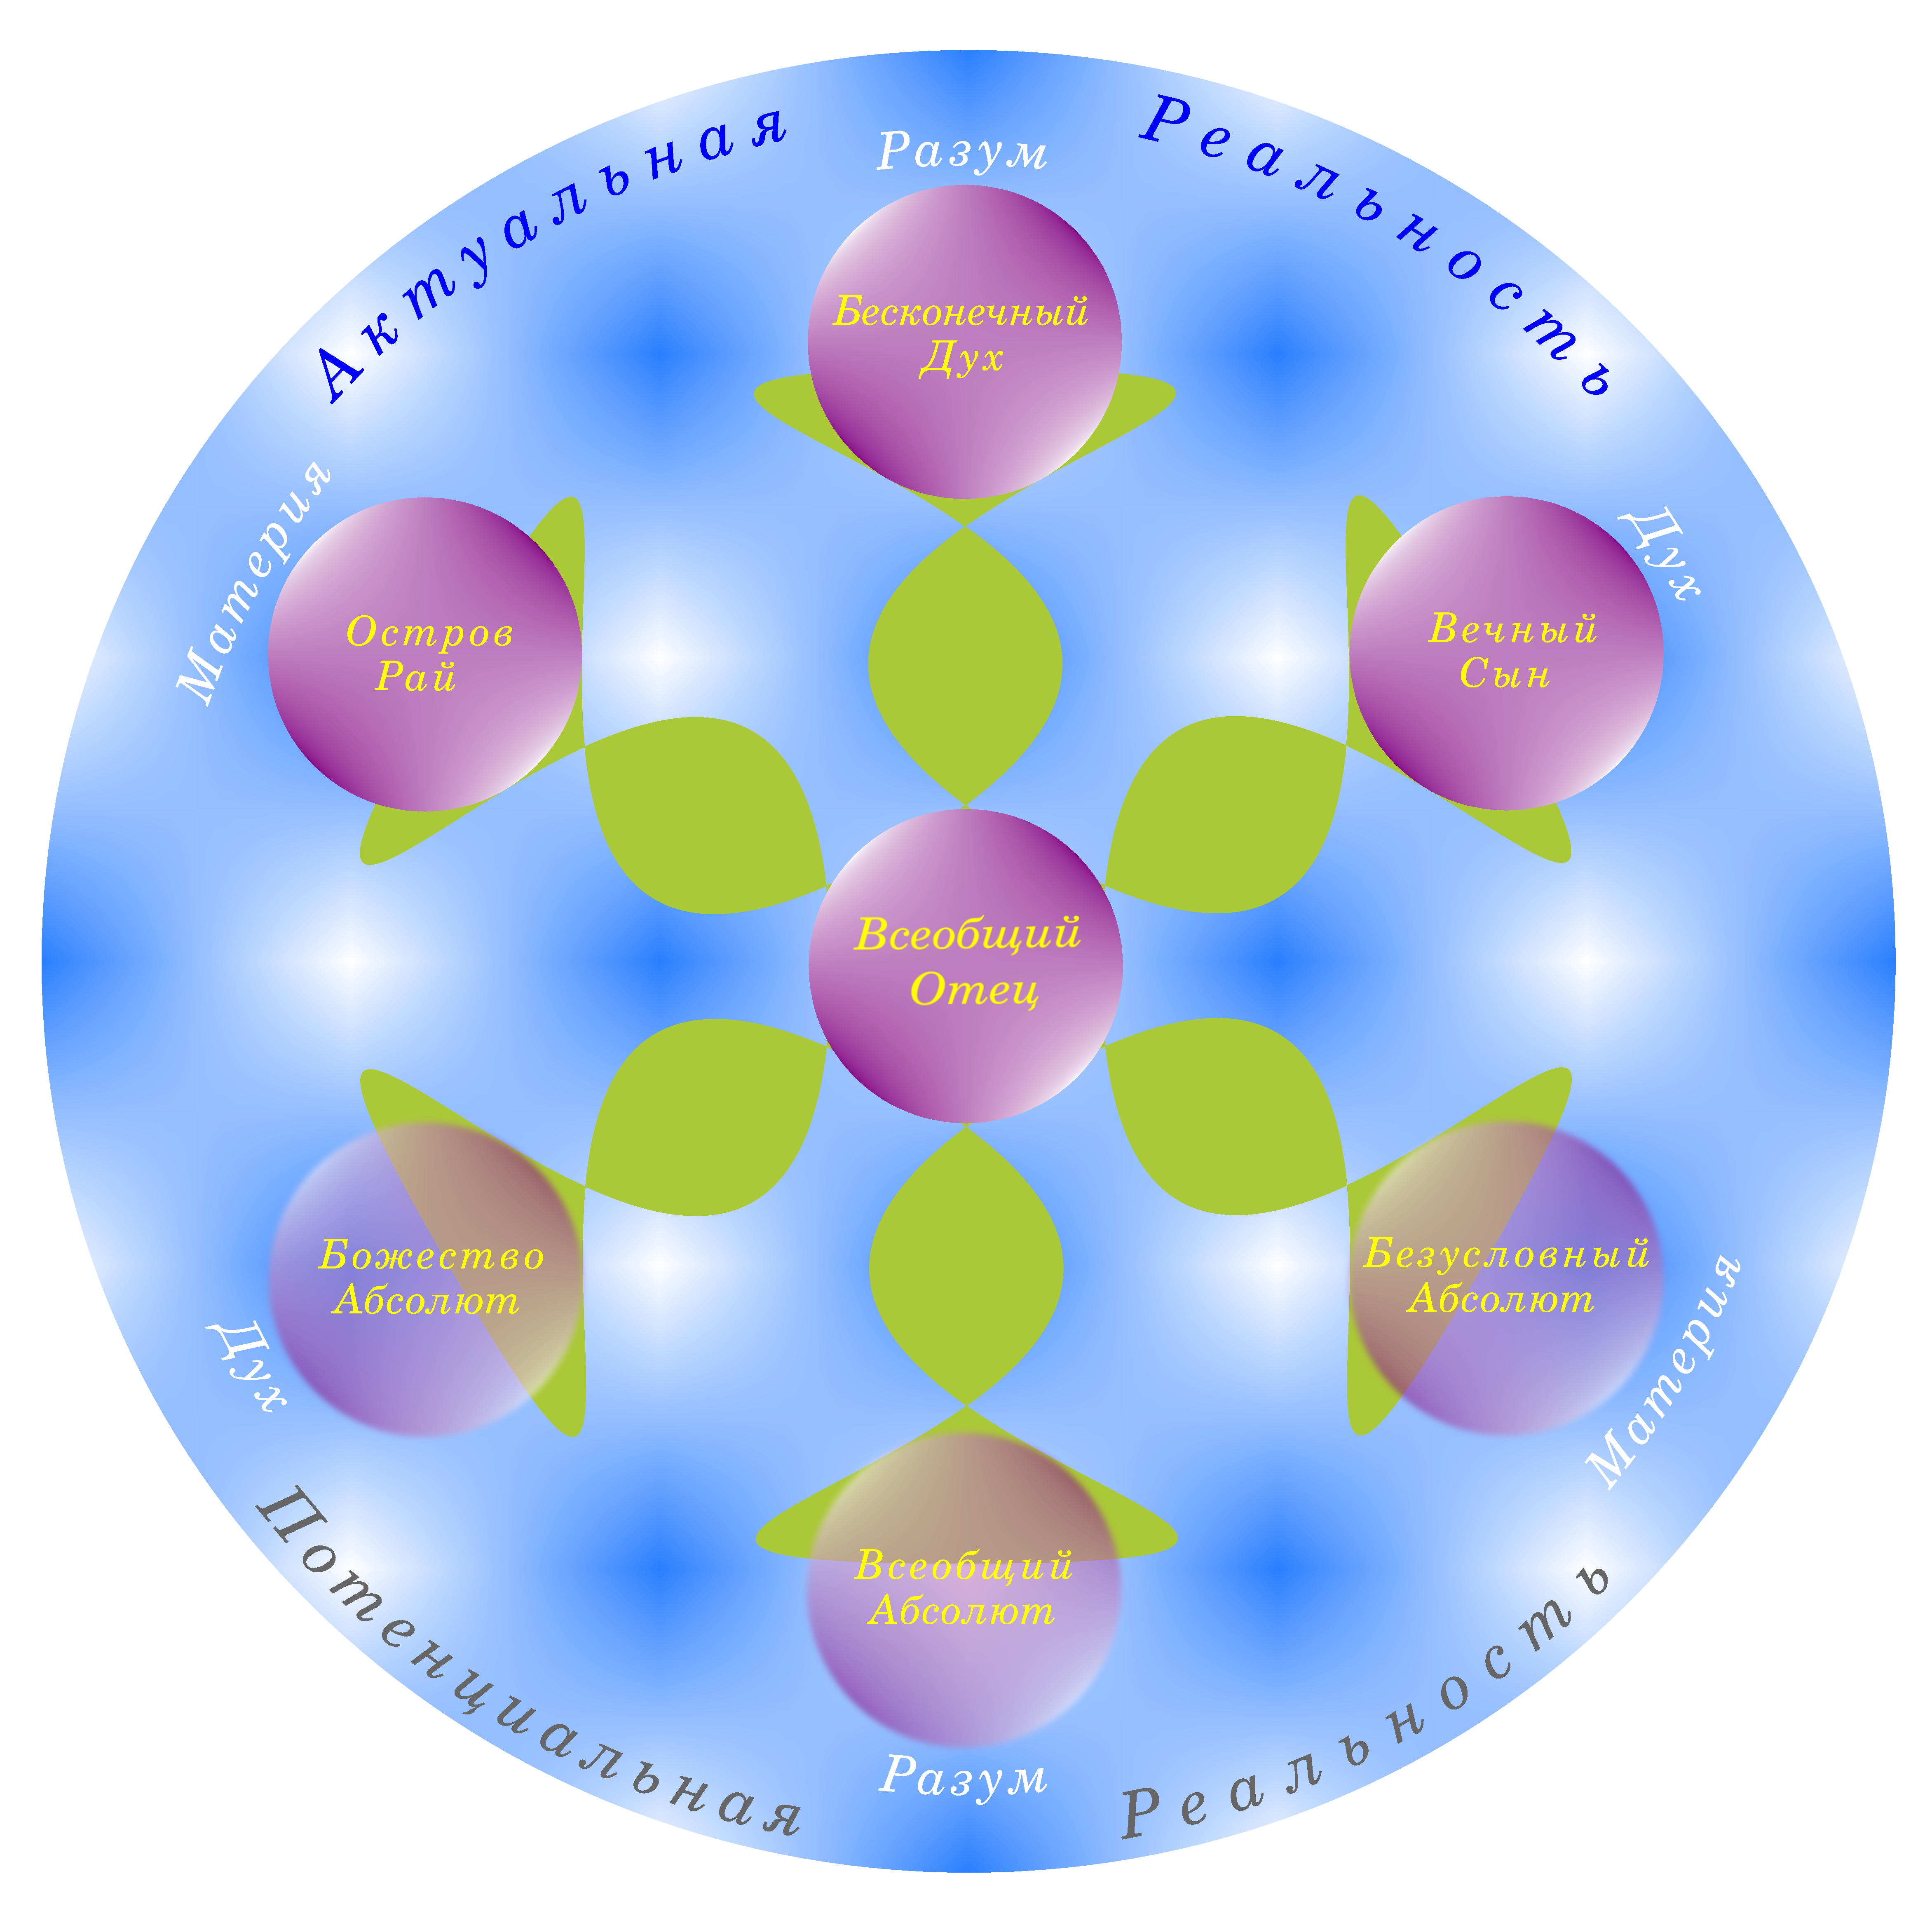
\includegraphics[width=0.95\columnwidth]{images/realnost.pdf}\caption{Семь Абсолютов и структура реальности}\end{figure}}
\vs p000 3:11 Следовательно, Первый Источник и Центр является первичным во всех областях: обожествлённых или необожествлённых, личностных или безличностных, актуальных или потенциальных, конечных или бесконечных. Никакая вещь или существо, никакая относительность или завершённость не существует иначе, как в прямом или косвенном отношении и в зависимости от первичности Первого Источника и Центра.
\vs p000 3:12 \pc \bibemph{Первый Источник и Центр} связан со вселенной следующим образом:
\vs p000 3:13 \ublistelem{1.}\bibnobreakspace Гравитационные силы материальных вселенных сходятся в гравитационном центре нижнего Рая. Именно поэтому географическое положение его личности\fnst{\textbf{его личности} То есть, личности Первого Источника и Центра --- Бога Отца.} навечно фиксировано в абсолютной связи с центром силы\hyp{}энергии нижней, или материальной, плоскости Рая. Но абсолютная личность\fnst{\textbf{абсолютная личность} Здесь использовано английское слово personality, в отличие от слова person, использованного в предыдущем предложении в фразе <<его личности>>. Слово person означает конкретного индивидуума, а personality --- это некий таинственный и невидимый дар Отца, интегрирующий в одно уникальное целое видимые материальные, моронтийные и духовные компоненты, из которых индивидуум состоит. Здесь, казалось бы, слово personality использовано в смысле person, но, по\hyp{}видимому, когда говорят об <<абсолютной личности Божества>>, имеется в виду не конкретный индивидуум (Вечный Сын), а максимальным образом обобщённая концепция <<абсолюта личности>>, и эта концепция, в некотором смысле, <<обитает>> на верхней плоскости Рая, воплощённая в конкретной личности\hyp{}индивидууме Вечного Сына.} Божества существует на верхней, или духовной, плоскости Рая.
\vs p000 3:14 \ublistelem{2.}\bibnobreakspace Силы разума сходятся в Бесконечном Духе; дифференцированный и дивергентный\fnst{\textbf{дифференцированный и дивергентный} То есть, разум, разделённый для каждой отдельной сверхвселенной на несовместимые (без переводчика --- Рая), но, в конечном счёте, дополняющие друг друга, контуры.} космический разум --- в Семи Главных Духах; фактуализующийся\fnst{\textbf{фактуализующийся} То есть, становящийся реальным, англ. factualizing.} разум Верховного как пространственно\hyp{}временн\'ой опыт --- в Мажестоне\fnst{\textbf{Мажестоне} В оригинале Majeston, вероятно, от английского Majesty --- Величие, Величество, Величественность.}.
\vs p000 3:15 \ublistelem{3.}\bibnobreakspace Вселенские силы духа сходятся в Вечном Сыне.
\vs p000 3:16 \ublistelem{4.}\bibnobreakspace Безграничная способность к божественному действию заключена в Божестве Абсолюте.
\vs p000 3:17 \ublistelem{5.}\bibnobreakspace Безграничная способность к отклику бесконечности\fnst{\textbf{отклику бесконечности} Или <<отклику на бесконечность>>, англ. infinity response.} существует в Безусловном Абсолюте.
\vs p000 3:18 \ublistelem{6.}\bibnobreakspace Два Абсолюта --- Условный и Безусловный --- координированы и объединены во Всеобщем Абсолюте и им же.
\vs p000 3:19 \ublistelem{7.}\bibnobreakspace Потенциальная личность эволюционного нравственного существа, или любого другого нравственного существа, сосредоточена в личности Всеобщего Отца.
\vs p000 3:20 \pc РЕАЛЬНОСТЬ, как она понимается конечными существами, является частичной, относительной и призрачной. Максимальная реальность Божества, полностью доступная пониманию эволюционных конечных созданий, заключена в пределах Верховного Существа. Тем не менее, существуют предшествующие и вечные реальности, сверхконечные реальности, которые являются исходными по отношению к этому Верховному Божеству эволюционных пространственно\hyp{}временн\'ых созданий. Пытаясь изобразить происхождение и природу вселенской реальности, мы вынуждены использовать метод пространственно\hyp{}временн\'ого рассуждения, чтобы дотянуться до уровня конечного разума. Поэтому многие одновременные события вечности должны быть представлены как последовательные действия.
\vs p000 3:21 С точки зрения пространственно\hyp{}временн\'ого создания на происхождение и дифференциацию Реальности, вечное и бесконечное Я ЕСТЬ достигло освобождения Божества от оков безусловной бесконечности посредством проявления врождённой и вечной свободной воли, и это отсоединение от безусловной бесконечности создало первое \bibemph{абсолютное напряжение божественности [divity\hyp{}tension]}. Это напряжение дифференциала бесконечности разрешается Всеобщим Абсолютом, который функционирует так, чтобы объединить и согласовать динамическую бесконечность Тотального Божества\index{Божество!Тотальное} и статическую бесконечность Безусловного Абсолюта.
\vs p000 3:22 В этом первоначальном акте теоретическое Я ЕСТЬ достигло реализации личности, становясь одновременно Вечным Отцом Изначального Сына и Вечным Источником Острова Рай. Сосуществуя с дифференциацией Сына от Отца, и в присутствии Рая, появились личность Бесконечного Духа и центральная вселенная Хавона. С появлением сосуществующего личностного Божества --- Вечного Сына и Бесконечного Духа --- Отец избежал как личность неизбежного, в противном случае, рассеивания по всему потенциалу Тотального Божества\index{Божество!Тотальное}. С тех пор, только в Троичной ассоциации с двумя равными ему Божествами, Отец заполняет весь потенциал Божества, в то время как эмпирическое Божество всё более актуализируется на уровнях божественности Верховности, Предельности и Абсолютности.
\vs p000 3:23 \pc \bibemph{Концепция Я ЕСТЬ} --- философская уступка, которую мы делаем связанному временем и скованному пространством конечному разуму человека, невозможности понимания созданием существований в вечности [eternity existences] --- не имеющих начала и конца реальностей и отношений. Для пространственно\hyp{}временн\'ого создания все вещи должны иметь начало, за исключением ОДНОГО БЕСПРИЧИННОГО --- первопричины причин. Поэтому мы и концептуализируем данный философский уровень\hyp{}ценность как Я ЕСТЬ, в то же время объясняя всем созданиям, что Вечный Сын и Бесконечный Дух со\hyp{}вечны с Я ЕСТЬ; иными словами, что никогда не было времени, когда Я ЕСТЬ не являлось \bibemph{Отцом} Сына и, вместе с ним, Духа.
\vs p000 3:24 \pc Термин \bibemph{Бесконечный} используется для обозначения полноты --- завершённости, подразумеваемой в первичности Первого Источника и Центра. \bibemph{Теоретическое} Я ЕСТЬ является расширением <<бесконечности воли>> в философии созданий, но Бесконечный есть \bibemph{актуальный} ценность\hyp{}уровень [value\hyp{}level], представляющий вечность\hyp{}напряжение\fnst{\textbf{вечность\hyp{}напряжение} Или напряжение вечности, англ. [eternity\hyp{}intension]} истинной бесконечности абсолютной и ничем не скованной свободной воли Всеобщего Отца. Эта концепция иногда обозначается как Отец\hyp{}Бесконечный.
\vs p000 3:25 Большая часть путаницы со стороны существ всех категорий --- как низших, так и высших, --- возникающая в их усилиях найти Отца\hyp{}Бесконечного, заложена в их ограничениях понимания. Абсолютная первичность Всеобщего Отца не очевидна на суббесконечных уровнях; поэтому вероятно, что только Вечный Сын и Бесконечный Дух действительно знают Отца как бесконечность; для всех других личностей такая концепция представляет собой проявление веры.
\usection{4.\bibnobreakspace ВСЕЛЕНСКАЯ РЕАЛЬНОСТЬ}
\vs p000 4:1 Реальность дифференциально\fnst{\textbf{дифференциально} То есть, <<по\hyp{}разному>>.} актуализируется на различных вселенских уровнях; реальность возникает во Всеобщем Отце и в результате его бесконечного волеизъявления; она реализуема в трёх первичных фазах на многих различных уровнях вселенской актуализации:
\vs p000 4:2 \ublistelem{1.}\bibnobreakspace \bibemph{Необожествлённая реальность} простирается от областей энергий неличностного до сфер реальности неперсонализируемых ценностей вселенского существования, вплоть до присутствия Безусловного Абсолюта.
\vs p000 4:3 \ublistelem{2.}\bibnobreakspace \bibemph{Обожествлённая реальность} охватывает все бесконечные потенциалы Божества\fnst{\textbf{бесконечные потенциалы Божества} Или <<потенциалы бесконечного Божества>>, англ. infinite Deity potentials.}, простирающиеся вверх через все сферы личности, от низшей конечной до высшей бесконечной, заключая в себе, таким образом, сферу всего того, что персонализируемо, и даже более того --- вплоть до присутствия Божества Абсолюта.
\vs p000 4:4 \ublistelem{3.}\bibnobreakspace \bibemph{Взаимосвязанная реальность}. Вселенская реальность является, предположительно, либо обожествлённой, либо необожествлённой, но для субобожествлённых существ, существует огромная область взаимосвязанной реальности, потенциальной и актуализирующейся, которую трудно идентифицировать. Большая часть этой координированной реальности заключена в пределах сфер Всеобщего Абсолюта.
\vs p000 4:5 Вот первичная концепция первоначальной реальности: Отец инициирует и поддерживает Реальность. Первичными \bibemph{дифференциалами} реальности являются обожествлённая и необожествлённая реальность --- Божество Абсолют и Безусловный Абсолют. Первичным \bibemph{отношением} является напряжение между ними. Это инициированное Отцом напряжение божественности совершенным образом разрешается Всеобщим Абсолютом и увековечивается в качестве него.
\vs p000 4:6 \pc С точки зрения времени и пространства реальность далее делится как:
\vs p000 4:7 \ublistelem{1.}\bibnobreakspace \bibemph{Актуальная и потенциальная}. Реальности, существующие в полноте выражения, в противоположность тем, которые несут в себе нераскрытую способность к росту. Вечный Сын есть абсолютная духовная актуальность; смертный человек является в очень значительной степени нереализованной духовной потенциальностью.
\vs p000 4:8 \ublistelem{2.}\bibnobreakspace \bibemph{Абсолютная и субабсолютная}. Абсолютные реальности это существования в вечности. Субабсолютные реальности проецируются на двух уровнях: абсониты\fnst{\textbf{абсониты} Вещи и существа абсонитного уровня реальности, англ. Absonites.} --- реальности, относительные в отношении как ко времени, так и к вечности; финиты\fnst{\textbf{финиты} Вещи и существа конечного уровня реальности, англ. Finites.} --- реальности, проецируемые в пространстве и актуализируемые во времени.
\vs p000 4:9 \ublistelem{3.}\bibnobreakspace \bibemph{Экзистенциальная и эмпирическая}. Райское Божество экзистенциально, но появляющиеся Верховное и Предельное являются эмпирическими.
\vs p000 4:10 \ublistelem{4.}\bibnobreakspace \bibemph{Личностная и безличностная}. Распространение Божества, выражение личности и вселенская эволюция навечно обусловлены актом свободной воли Отца, навсегда отделившим разумно\hyp{}духовно\hyp{}личностные смыслы и ценности актуальности и потенциальности, сосредоточенные в Вечном Сыне, от тех вещей, которые сосредоточены в Острове Рай и присущи ему.
\vs p000 4:11 \pc РАЙ --- это термин, включающий личностные и неличностные фокальные\fnst{\textbf{фокальные} То есть, являющиеся фокусами чего\hyp{}то, например, контуров абсолютной гравитации.} Абсолюты всех фаз вселенской реальности. Рай, правильно определённый, может обозначать любую и все формы реальности, Божества, божественности, личности и энергии --- духовные, ментальные или материальные. Все разделяют Рай, как место происхождения, функции и предназначения, касательно ценностей, смыслов и фактического существования.
\vs p000 4:12 \pc \bibemph{Остров Рай} --- Рай, не определённый иначе, --- это Абсолют материально\hyp{}гравитационного контроля Первого Источника и Центра. Рай неподвижен, будучи единственным стационарным объектом во вселенной вселенных. Остров Рай имеет вселенское расположение, но не имеет положения в пространстве. Этот вечный Остров является действительным источником физических вселенных --- прошлых, настоящих и будущих. Ядерный Остров Света [The nuclear Isle of Light] является производным Божества, но едва ли сам является Божеством; не являются и материальные творения частью Божества; они --- его следствие.
\vs p000 4:13 Рай --- не создатель; он есть уникальный регулятор многих видов вселенской деятельности, гораздо в большей степени регулятор, чем реактор. По всем материальным вселенным Рай оказывает влияние на реакцию и поведение всех существ, имеющих отношение к силе, энергии и мощи, но сам Рай уникален, исключителен и изолирован во вселенных. Рай не символизирует ничего и ничто не символизирует Рай. Он --- ни сила, ни присутствие; он просто --- \bibemph{Рай}.
\usection{5.\bibnobreakspace ЛИЧНОСТНЫЕ РЕАЛЬНОСТИ}
\vs p000 5:1 Личность --- это уровень обожествлённой реальности и простирается от уровня смертных и промежуточных созданий более высокой активации разума в поклонении и мудрости, через моронтийный и духовный, вплоть до достижения завершённости статуса личности. Таково эволюционное восхождение личности смертного и родственного ему создания, но существует множество других типов вселенских личностей.
\vs p000 5:2 Реальность подвержена всеобщему распространению, личность --- бесконечному умножению разнообразия, и обе они способны к почти неограниченной координации с Божеством и вечной стабилизации. Тогда как метаморфический диапазон неличностной реальности определённо ограничен, мы не знаем никаких ограничений для постепенной эволюции личностных реальностей.
\vs p000 5:3 На достигнутых эмпирических уровнях все личностные типы или ценности способны к содружеству и даже к совместному созиданию. Даже Бог и человек могут сосуществовать в объединённой личности, что с таким изяществом демонстрируется в нынешнем статусе Христа Михаила --- Сына Человеческого и Сына Божьего.
\vs p000 5:4 Все суббесконечные типы и фазы личности ассоциативно достижимы и являются потенциально совместно созидательными. Доличностное, личностное и сверхличностное --- всех их связывает взаимная потенциальная возможность координированного достижения [attainment], прогрессивного достижения [achievement]\fnst{\textbf{[attainment]\ldots [achievement]} Разница заключается в том, что под <<прогрессивным достижением>> имеется в виду достижение заданных заранее уровней, например, <<кругов развития>>, а под <<координированным достижением>> подразумевается обоюдное достижение чего-либо, невозможное друг без друга, например: достижение личности Настройщиком, а бессмертия --- душой человека.} и со\hyp{}творчества. Но никогда безличностное не превращается непосредственно в личностное. Личность никогда не возникает спонтанно; она является даром Райского Отца. Личность накладывается на энергию и ассоциируется только с живыми энергетическими системами; индивидуальность [identity] может ассоциироваться с неживыми энергетическими образцами [patterns].
\vs p000 5:5 \pc Всеобщий Отец\index{Бог!Всеобщий Отец} есть тайна реальности личности, дарования личности и предназначения личности. Вечный Сын есть абсолютная личность, тайна духовной энергии, моронтийных духов и духов, ставших совершенными. Совместный Вершитель есть духовно\hyp{}р\'азумная [spirit\hyp{}mind] личность, источник дара понимания [intelligence], способности рассуждения [reason] и вселенского разума. Однако Остров Рай является неличностным и внедуховным, будучи сущностью вселенского тела, источником и центром физической материи и абсолютным главным образцом вселенской материальной реальности.
\vs p000 5:6 \pc Эти качества вселенской реальности проявляются в человеческом опыте на Урантии на следующих уровнях:
\vs p000 5:7 \ublistelem{1.}\bibnobreakspace \bibemph{Тело}\index{человек!тело|textbf}. Материальный, или физический, организм человека. Живой электрохимический механизм животной природы и происхождения.
\vs p000 5:8 \ublistelem{2.}\bibnobreakspace \bibemph{Разум}\index{человек!разум|textbf}. Механизм мышления, восприятия и чувств человеческого организма. Весь сознательный и бессознательный опыт. Интеллект, связанный с эмоциональной жизнью, стремящийся вверх через поклонение и мудрость к уровню духа.
\vs p000 5:9 \ublistelem{3.}\bibnobreakspace \bibemph{Дух}\index{человек!дух|textbf}. Божественный дух, обитающий в разуме человека, --- Настройщик Мышления. Этот бессмертный дух является доличностным --- он не личность, хотя и предназначен для того, чтобы стать частью личности выживающего\fnst{\textbf{выживающего} Иными словами, <<продолжающего существование>> или <<сохранившегося после смерти>>, англ. surviving.} смертного создания.
\vs p000 5:10 \ublistelem{4.}\bibnobreakspace \bibemph{Душа}\index{человек!душа|textbf}. Душа человека есть эмпирическое приобретение. Когда смертное создание выбирает <<исполнять волю небесного Отца>>, пребывающий в нём дух становится отцом \bibemph{новой реальности} в человеческом опыте. Смертный и материальный разум является матерью\fnst{\textbf{материальный разум является матерью} Оба английских слова matter (материя) и mother (мать) имеют одинаковое происхождение, а именно, от греческого слова \textgreek{μήτηρ} (мать).} этой же самой возникающей реальности. Субстанция этой новой реальности ни материальна, ни духовна --- она \bibemph{моронтийна}. Это --- появляющаяся и бессмертная душа, которой предназначено пережить смерть смертного [mortal death] и начать Райское восхождение.
\vs p000 5:11 \pc \bibemph{Личность}\index{человек!личность|textbf}. Личность смертного человека не является ни телом, ни разумом, ни духом; не является также она душой. Личность есть единственная неизменная реальность во всём остальном постоянно изменяющемся опыте создания; и она объединяет все остальные связанные факторы индивидуальности. Личность --- это уникальный дар, которым Всеобщий Отец\index{Бог!Всеобщий Отец} наделяет живые и связанные друг с другом энергии материи, разума и духа, и которая выживает с выживанием моронтийной души.
\vs p000 5:12 \pc \bibemph{Моронтия} --- термин, обозначающий громадный промежуточный уровень между материальным и духовным. Он может обозначать личностные или безличностные реальности, живые или неживые энергии. Продольные нити моронтийной ткани\fnst{\textbf{моронтийной ткани} Термин <<моронтия>> является композитным словом, составленным из слов <<материя>> и <<мораль>>. Помимо личного опыта редактора обоснование приводится в сноске к \bibref[112:3.2]{p112 3:2}.} --- духовны, поперечные --- материальны.
\usection{6.\bibnobreakspace ЭНЕРГИЯ И ОБРАЗЕЦ}
\vs p000 6:1 Всё и вся, что реагирует на личностный контур Отца, мы называем личностным\index{личность|textbf}. Всё и вся, что реагирует на духовный контур Сына, мы называем духом\index{дух|textbf}. Всё и вся, что реагирует на контур разума Совместного Вершителя, мы называем разумом,\index{разум|textbf} понимаемым как атрибут Бесконечного Духа, --- разумом во всех его фазах. Всё и вся, что реагирует на материально\hyp{}гравитационный контур с центром в нижнем Раю, мы называем материей\index{материя|textbf} --- энергией\hyp{}материей\index{материя!энергия\hyp{}материя|textbf} во всех её метаморфических состояниях.
\vs p000 6:2 \pc ЭНЕРГИЯ\index{энергия|textbf} используется нами как всеобъемлющий термин, применяемый к духовным, ментальным и материальным сферам. Так же широко используется слово \bibemph{сила}. Термин \bibemph{мощь}\index{мощь|textbf} [power] обычно ограничен обозначением электронного уровня вещества, то есть материи, реагирующей на линейную гравитацию в большой вселенной. Этим же словом [power] обозначается полновластие [sovereignty]. Мы не можем следовать вашим общепринятым определениям силы, энергии и мощи. Язык настолько скуден, что мы вынуждены придавать этим терминам множественный смысл.
\vs p000 6:3 \pc \bibemph{Физическая энергия}\index{энергия!физическая|textbf} --- термин, обозначающий все фазы и формы наблюдаемого движения, действия и потенциала.
\vs p000 6:4 При обсуждении физико\hyp{}энергетических проявлений мы, обычно, применяем термины: космическая сила, появляющаяся энергия и вселенская мощь. Они часто употребляются следующим образом:
\vs p000 6:5 \ublistelem{1.}\bibnobreakspace \bibemph{Космическая сила}\index{энергия!космическая сила|textbf} охватывает все виды энергии, происходящие от Безусловного Абсолюта, но пока не реагирующие на Райскую гравитацию.
\vs p000 6:6 \ublistelem{2.}\bibnobreakspace \bibemph{Появляющаяся энергия}\index{энергия!появляющаяся|textbf} охватывает все виды энергии, которые реагируют на Райскую гравитацию, но пока не реагируют на локальную, или линейную, гравитацию. Это предэлектронный уровень энергии\hyp{}материи.
\vs p000 6:7 \ublistelem{3.}\bibnobreakspace \bibemph{Вселенская мощь}\index{энергия!вселенская мощь|textbf} включает все формы энергии, которые, хоть и реагируют на Райскую гравитацию, напрямую чувствительны к линейной гравитации. Это электронный уровень энергии\hyp{}материи и все её последующие модификации [evolutions].
\vs p000 6:8 \pc \bibemph{Разум} есть феномен, подразумевающий присутствие\hyp{}действие [presence\hyp{}activity] \bibemph{живого служения} в дополнение к различным энергетическим системам; и это верно на всех уровнях интеллекта. В личности разум всегда находится между духом и материей; поэтому вселенная освещается тремя видами света: материальным светом, интеллектуальным прозрением и духовным сиянием.
\vs p000 6:9 \pc \bibemph{Свет}\index{свет|textbf} --- сияние духа --- есть словесный символ, фигура речи, которая означает личностное проявление, характерное для духовных существ различных классов. Это сияющее излучение ни в коей мере не связано ни с интеллектуальным прозрением, ни с физически\hyp{}световыми [physical\hyp{}light] проявлениями.
\vs p000 6:10 \pc ОБРАЗЕЦ\index{образец|textbf} [PATTERN] может проецироваться как материальная, духовная или ментальная энергия, либо как любая их комбинация. Он может пропитывать [pervade] личности, индивидуальности, сущности или неживую материю. Однако образец есть образец и остаётся образцом; только \bibemph{копии} множатся.
\vs p000 6:11 Образец может конфигурировать энергию, но не управляет ею. Только гравитация управляет энергией\hyp{}материей. Ни пространство,\index{пространство} ни образец не реагируют на гравитацию, однако между пространством и образцом нет никакой связи: пространство не является ни образцом, ни потенциальным образцом. Образец есть конфигурация реальности, которая уже выплатила весь гравитационный долг;\index{гравитация!гравитационный долг|textbf} \bibemph{реальность}\index{реальность} любого образца состоит из его энергий, его разума, духа или материальных компонент.
\vs p000 6:12 В отличие от \bibemph{общего} аспекта, образец раскрывает \bibemph{индивидуальный} аспект энергии и личности. Формы личности или индивидуальности это образцы, проистекающие из энергии (физической, духовной или ментальной), но они не присущи ей внутренне. То качество энергии или личности, благодаря которому возникает образец, может быть приписано Богу --- Божеству --- наделению Райской силой, сосуществованию личности и мощи.
\vs p000 6:13 Образец --- это главная схема, с которой делаются все копии. Вечный Рай есть абсолют образцов; Вечный Сын есть образец личности; Всеобщий Отец\index{Бог!Всеобщий Отец} есть  прямой предок\hyp{}источник обоих. Но Рай не дарует образец, а Сын не может даровать личность.
\usection{7.\bibnobreakspace ВЕРХОВНОЕ СУЩЕСТВО}
\vs p000 7:1 Механизм Божества главной вселенной двоякий касательно отношений в вечности. Бог Отец, Бог Сын и Бог Дух являются вечными --- экзистенциальными существами, в то время как Бог Верховный, Бог Предельный и Бог Абсолютный --- \bibemph{актуализирующиеся} личности Божества пост\hyp{}Хавонских эпох в пространственно\hyp{}временн\'ых и превосходящих пространство\hyp{}время сферах эволюционного расширения главной вселенной. Эти актуализирующиеся личности Божества являются вечными по отношению к будущему --- со времени, когда (и как) они синтезируют мощь и личность [power\hyp{}personalize] в растущих вселенных с помощью метода эмпирической актуализации ассоциативно\hyp{}созидательных потенциалов вечных Райских Божеств.
\vs p000 7:2 Следовательно, присутствие Божества двойственно:
\vs p000 7:3 \ublistelem{1.}\bibnobreakspace \bibemph{Экзистенциальное}\index{Божество!экзистенциальное|textbf} --- существа, вечного существования --- прошлого, настоящего и будущего.
\vs p000 7:4 \ublistelem{2.}\bibnobreakspace \bibemph{Эмпирическое}\index{Божество!эмпирическое|textbf} --- существа, актуализирующиеся в пост\hyp{}Хавонском настоящем, но существование которых не имеет конца во всей будущей вечности.
\vs p000 7:5 \pc Отец, Сын и Дух экзистенциальны --- экзистенциальны в актуальности (хотя все потенциалы являются, предположительно, эмпирическими). Верховный и Предельный --- целиком эмпирические. Божество Абсолют является эмпирическим в актуализации, но экзистенциальным в потенциальности. Сущность Божества вечна, но только три изначальных лица Божества являются безусловно вечными. Все другие личности Божества имеют начало, но они вечны в предназначении.
\vs p000 7:6 Достигнув экзистенциального самовыражения Божества в Сыне и Духе, Отец теперь достигает эмпирического выражения на доселе неличностных и нераскрытых уровнях божества --- как Бог Верховный, Бог Предельный и Бог Абсолютный; но эти эмпирические Божества сейчас не вполне существуют; они находятся в процессе актуализации.
\vs p000 7:7 \pc \bibemph{Бог Верховный}\index{Бог!Верховный|textbf} в Хавоне есть личностное духовное отражение триединого Райского Божества. В настоящее время это ассоциативное отношение Божества претерпевает созидательное расширение наружу в Боге Семичастном и синтезируется в эмпирическую мощь Всемогущего Верховного в большой вселенной. Таким образом, Райское Божество, экзистенциальное в трёх лицах, эмпирически эволюционирует в двух фазах Верховности, в то время как эти дуальные фазы объединяют мощь и личность [power\hyp{}personality unifying] в одного Господа --- Верховное Существо.
\vs p000 7:8 Всеобщий Отец\index{Бог!Всеобщий Отец} в акте свободной воли достигает освобождения от уз бесконечности и оков вечности путём тринитизации --- тройной персонализации Божества. Верховное Существо даже сейчас эволюционирует как субвечное личностное объединение семичастного проявления Божества в пространственно\hyp{}временн\'ых сегментах большой вселенной.
\vs p000 7:9 \pc \bibemph{Верховное Существо} не является непосредственным создателем (за исключением того, что оно является отцом Мажестона), но оно --- координатор, синтезирующий всю вселенскую деятельность, объединяющую создания и Создателя. Верховное Существо, ныне актуализирующееся в эволюционных вселенных, есть Божество, коррелирующее и синтезирующее пространственно\hyp{}временн\'ую божественность --- триединого Божества Рая\fnst{\textbf{триединого Божества Рая} То есть, <<божественность триединого Божества Рая>> и т.д.} в эмпирической ассоциации с Верховными Создателями времени и пространства. Окончательно актуализированное это эволюционное Божество будет представлять собой вечное слияние конечного и бесконечного --- вечный и нерасторжимый союз эмпирической мощи и духовной личности.
\vs p000 7:10 Под направляющим побуждением эволюционирующего Верховного Существа вся пространственно\hyp{}временн\'ая конечная реальность вовлечена во всё возрастающую [ever\hyp{}ascending] мобилизацию и всё более совершенное объединение (синтез мощи и личности) всех фаз и ценностей конечной реальности, в ассоциации с различными фазами Райской реальности, с целью и намерением впоследствии предпринять попытку дотянуться до абсонитных уровней достижения сверхсозданий.
\usection{8.\bibnobreakspace БОГ СЕМИЧАСТНЫЙ}
\vs p000 8:1 Чтобы искупить конечность статуса и компенсировать концептуальную ограниченность создания, Всеобщий Отец\index{Бог!Всеобщий Отец} установил семиступенчатый подход эволюционного создания к Божеству:
\vs p000 8:2 \ublistelem{1.}\bibnobreakspace Райские Сыны Создатели.
\vs p000 8:3 \ublistelem{2.}\bibnobreakspace Ветхие Днями.
\vs p000 8:4 \ublistelem{3.}\bibnobreakspace Семь Главных Духов.
\vs p000 8:5 \ublistelem{4.}\bibnobreakspace Верховное Существо.
\vs p000 8:6 \ublistelem{5.}\bibnobreakspace Бог Дух.
\vs p000 8:7 \ublistelem{6.}\bibnobreakspace Бог Сын.
\vs p000 8:8 \ublistelem{7.}\bibnobreakspace Бог Отец.
\vs p000 8:9 \pc Эта семикратная персонализация Божества во времени и пространстве и для семи сверхвселенных позволяет смертному человеку достигнуть присутствия Бога, который есть дух. Это семичастное Божество, которое --- по отношению к конечным пространственно\hyp{}временн\'ым созданиям --- когда\hyp{}нибудь в будущем, в результате синтеза мощи и личности, превратится в Верховное Существо, является функциональным Божеством смертных эволюционных созданий, восходящих к Раю. Такое эмпирическое открытие\hyp{}продвижение к реализации Бога начинается с признания божественности Сына Создателя локальной вселенной и, через Ветхих Днями сверхвселенной и посредством личности одного из Семи Главных Духов, приводит к достижению открытия и признания божественной личности Всеобщего Отца в Раю.
\vs p000 8:10 \pc Большая вселенная --- это область трёхчастного Божества: Троицы Верховности, Бога Семичастного и Верховного Существа. Бог Верховный потенциален в Райской Троице, от которой он получает свою личность и атрибуты духа; однако сейчас он актуализируется в Сынах Создателях, Ветхих Днями и в Главных Духах, от которых он получает свою мощь как Всемогущий для сверхвселенных времени и пространства. Это проявление мощи непосредственного Бога эволюционных созданий фактически эволюционирует во времени и пространстве одновременно с ними. Всемогущий Верховный, эволюционирующий на ценностном уровне [value\hyp{}level] неличностной деятельности, и духовное лицо Бога Верховного есть \bibemph{одна реальность} --- Верховное Существо\index{Верховное Существо}.
\vs p000 8:11 Объединённые в Божестве Бога Семичастного, Сыны Создатели предоставляют механизм, благодаря которому смертный становится бессмертным, и конечное достигает объятий бесконечного. Верховное Существо предоставляет метод мобилизации мощи и личности, божественного синтеза, \bibemph{всех} этих разнообразных процессов, таким образом позволяя конечному достичь абсонитного и, через другие возможные в будущем актуализации, попытаться достичь Предельного. Сыны Создатели и их Божественные Помощницы являются участниками этой верховной мобилизации, но Ветхие Днями и Семь Главных Духов, вероятно, навечно закреплены в качестве постоянных администраторов большой вселенной.
\vs p000 8:12 Функционирование Бога Семичастного начинается с организации семи сверхвселенных, и, вероятно, оно будет расширяться в связи с будущей эволюцией творений внешнего пространства. Организация этих будущих вселенных первичного, вторичного, третичного и четвертичного пространственных уровней прогрессивной эволюции несомненно ознаменует собой открытие [inauguration] трансцендентного и абсонитного приближения к Божеству.
\usection{9.\bibnobreakspace БОГ ПРЕДЕЛЬНЫЙ}
\vs p000 9:1 Подобно тому, как Верховное Существо постепенно эволюционирует из предшествующего дара божественности, заключённого в потенциале энергии и личности большой вселенной, так и Бог Предельный возникает из потенциалов божественности, находящихся в областях главной вселенной, превосходящих время и пространство. Актуализация Предельного Божества знаменует собой абсонитное объединение первой эмпирической Троицы и означает объединяющее распространение Божества на втором уровне творческой самореализации. Это составляет личностно\hyp{}мощностной эквивалент вселенской актуализации в эмпирическом Божестве абсонитных ценностей Рая на возникающих уровнях ценностей, превосходящих время и пространство. Завершение такого эмпирического раскрытия призвано предоставить предельное служение\hyp{}предназначение для всех пространственно\hyp{}временн\'ых созданий, достигших абсонитных уровней через завершённую реализацию Верховного Существа и благодаря помощи Бога Семичастного.
\vs p000 9:2 \pc \bibemph{Бог Предельный}\index{Бог!Предельный|textbf} обозначает личностное Божество, функционирующее на уровнях божественности абсонитного и на вселенских сферах сверхвремени и превзойдённого пространства. Предельный есть сверхверховное возникновение Божества. Верховный есть объединение Троицы, понимаемое конечными существами; Предельный есть объединение Райской Троицы, понимаемое абсонитными существами.
\vs p000 9:3 Всеобщий Отец\index{Бог!Всеобщий Отец} с помощью механизма эволюционного Божества фактически вовлечён в колоссальный и удивительный \bibemph{акт} фокализации личности и мобилизации мощи на соответствующих вселенских смысловых уровнях ценностей божественной реальности конечного, абсонитного и даже абсолютного.
\vs p000 9:4 Первые три, и вечные в прошлом, Божества Рая --- Всеобщий Отец,\index{Бог!Всеобщий Отец} Вечный Сын\index{Бог!Вечный Сын} и Бесконечный Дух\index{Бог!Бесконечный Дух} --- должны в вечном будущем быть личностно дополнены эмпирической актуализацией ассоциированных\fnst{\textbf{ассоциированных} То есть, связанных, как между собой, так и с экзистенциальными Божествами Рая.} эволюционных Божеств --- Богом Верховным, Богом Предельным и, возможно, Богом Абсолютным.
\vs p000 9:5 \pc Бог Верховный и Бог Предельный, теперь эволюционирующие в эмпирических вселенных, не являются экзистенциальными --- не прошлыми вечностями, только будущими вечностями; это обусловленные временем и пространством и трансцендентально\hyp{}обусловленные вечности. Они являются Божествами верховных, предельных и, возможно, верховно\hyp{}предельных способностей, но они испытали историческое вселенское происхождение. У них никогда не будет конца, но они имеют начало как личности. Они в самом деле являются актуализациями вечных и бесконечных потенциалов Божества, но сами они не являются ни безусловно вечными, ни бесконечными.
\usection{10.\bibnobreakspace БОГ АБСОЛЮТНЫЙ}
\vs p000 10:1 Есть много черт вечной реальности \bibemph{Божества Абсолюта}, которые невозможно полностью объяснить пространственно\hyp{}временн\'ому конечному разуму, но актуализация \bibemph{Бога Абсолютного} будет следствием объединения второй эмпирической Троицы --- Абсолютной Троицы. Это составит эмпирическую реализацию абсолютной божественности, объединение абсолютных смыслов на абсолютных уровнях; но мы не уверены касательно охвата всех абсолютных ценностей, ибо нам никогда не информировали о том, что Условный Абсолют эквивалентен Бесконечному. Сверхпредельные предназначения связаны с абсолютными смыслами и бесконечной духовностью, а без этих двух недостигнутых реальностей мы не можем установить абсолютные ценности.
\vs p000 10:2 Бог Абсолютный есть цель реализации\hyp{}достижения [realization\hyp{}attainment goal] всех сверхабсонитных существ, но потенциал мощи и личности Божества Абсолюта выходит за пределы нашего представления, и мы не решаемся обсуждать те реальности, которые столь далеко отстоят от эмпирической актуализации.
\usection{11.\bibnobreakspace ТРИ АБСОЛЮТА}
\vs p000 11:1 Когда объединённая мысль Всеобщего Отца и Вечного Сына, функционирующая в Боге Действия, воплотилась в создании божественной и центральной вселенной, Отец последовал за выражением своей мысли в слово Сына и акт их Совместного Исполнителя, отделив своё присутствие в Хавоне от потенциалов бесконечности. И эти нераскрытые потенциалы бесконечности остаются пространственно скрытыми [space concealed] в Безусловном Абсолюте и божественно покрытыми [enshrouded] в Божестве Абсолюте, в то время как оба они\fnst{\textbf{оба они} То есть два Абсолюта.} становятся одним в функционировании Всеобщего Абсолюта --- нераскрытой бесконечности\hyp{}единства Райского Отца.
\vs p000 11:2 Как потенция космической силы, так и потенция силы духа находятся в процессе постепенного откровения\hyp{}реализации, по мере обогащения всей реальности благодаря эмпирическому росту и за счёт корреляции эмпирического и экзистенциального Всеобщим Абсолютом. Благодаря уравновешивающему присутствию Всеобщего Абсолюта, Первый Источник и Центр реализует расширение эмпирического могущества, испытывает идентификацию со своими эволюционными созданиями и достигает распространения эмпирического Божества на уровнях Верховности, Предельности и Абсолютности.
\vs p000 11:3 \pc Когда невозможно полностью отличить Божество Абсолют от Безусловного Абсолюта, их предположительно комбинированная функция или координированное присутствие приписывается действию Всеобщего Абсолюта.
\vs p000 11:4 \pc \ublistelem{1.}\bibnobreakspace \bibemph{Божество Абсолют} представляется наимощнейшим активатором, в то время как Безусловный Абсолют предстаёт как наиэффективнейший механизатор\fnst{\textbf{механизатор} Англ. mechanizer, вероятно, означающее здесь <<источник чисто механических потенциальных возможностей>>.} в высшей степени объединённой и предельно координированной вселенной вселенных и даже великого множества вселенных, созданных, создаваемых и которые ещё будут созданы.
\vs p000 11:5 Божество Абсолют не может или, по крайней мере, не реагирует на какую\hyp{}либо вселенскую ситуацию субабсолютным образом. Каждая реакция этого Абсолюта на любую данную ситуацию кажется действующей во благо всех созданных вещей и существ --- не только в их настоящем состоянии существования, но и с точки зрения бесконечных возможностей всей будущей вечности.
\vs p000 11:6 Божество Абсолют --- это тот потенциал, который был сегрегирован от тотальной, бесконечной реальности добровольным выбором Всеобщего Отца и внутри которого происходят все типы божественной деятельности --- экзистенциальной и эмпирической. Это \bibemph{Условный Абсолют} в отличие от \bibemph{Безусловного Абсолюта;} но Всеобщий Абсолют\index{Абсолют!Всеобщий Абсолют} супераддитивен\fnst{\textbf{супераддитивен} То есть, представляет собой нечто б\'ольшее, чем простая сумма.} к обоим в охвате всего абсолютного потенциала.
\vs p000 11:7 \pc \ublistelem{2.}\bibnobreakspace \bibemph{Безусловный Абсолют} является неличностным, внебожественным и необожествлённым. Следовательно, Безусловный Абсолют лишён личности, божественности и всех прерогатив создателя. Ни факт, ни истина, ни опыт, ни откровение, ни философия, ни абсонитность [absonity] не способны проникнуть в природу и характер этого Абсолюта, не имеющего вселенской обусловленности.
\vs p000 11:8 Да будет ясно, что Безусловный Абсолют есть \bibemph{позитивная реальность,} наполняющая большую вселенную и, по\hyp{}видимому, простирающаяся с равным пространственным присутствием далее, в область силовых проявлений и доматериальных эволюций за пределами семи сверхвселенных в регионах пространства, потрясающих воображение своей протяжённостью. Безусловный Абсолют --- это не просто философская концепция негативизма, опирающаяся на допущения метафизической софистики касательно всеобщности, доминирования и первичности необусловленного и безусловного. Безусловный Абсолют является реальным вселенским сверхрегулированием в бесконечности; это сверхрегулирование безгранично в пространственно\hyp{}силовом смысле, но оно определённо обусловлено присутствием жизни, разума, духа и личности, и дополнительно обусловлено реакциями воли [will\hyp{}reactions] и целенаправленными мандатами Райской Троицы.
\vs p000 11:9 Мы убеждены, что Безусловный Абсолют не является недифференцированным и всепроникающим\fnst{\textbf{всепроникающим} Или <<все\hyp{}насыщающим>>, англ. all\hyp{}pervading.} влиянием, сравнимым либо с пантеистическими концепциями метафизики, либо с некогда бытовавшей в науке гипотезой эфира. Безусловный Абсолют не ограничен в силе и обусловлен Божеством, однако мы не вполне осознаём связь этого Абсолюта с духовными реальностями вселенных.
\vs p000 11:10 \pc \ublistelem{3.}\bibnobreakspace Мы логически заключаем, что \bibemph{Всеобщий Абсолют}\index{Абсолют!Всеобщий Абсолют} был неизбежным в абсолютном добровольном акте Всеобщего Отца --- дифференциации вселенских реальностей на обожествлённые и необожествлённые --- персонализуемые и неперсонализуемые --- ценности. Всеобщий Абсолют\index{Абсолют!Всеобщий Абсолют} есть феномен Божества, указывающий на разрешение напряжения, созданного добровольным актом дифференциации вселенской реальности, и функционирует как ассоциативный координатор этих итогов [these sum totals] экзистенциальных потенциальных возможностей.
\vs p000 11:11 \pc Напряжение\hyp{}присутствие Всеобщего Абсолюта означает выравнивание дифференциала между реальностью божества\fnst{\textbf{реальностью божества} Или <<божественной реальностью>>, англ. deity reality.} и необожествлённой реальностью, свойственного отделению динамики божественности свободы воли от статики безусловной бесконечности.
\vs p000 11:12 \pc Всегда помните: Потенциальная бесконечность абсолютна и неотделима от вечности. Актуальная бесконечность во времени может быть только частичной и, следовательно, должна быть неабсолютной; так же и бесконечность актуальной личности не может быть абсолютной, кроме как в безусловном Божестве. Именно дифференциал между потенциалом бесконечности в Безусловном Абсолюте и Божестве Абсолюте увековечивает Всеобщий Абсолют\fnst{\textbf{дифференциал \ldots\ увековечивает Всеобщий Абсолют} То есть, именно Всеобщий Абсолют увековечивается дифференциалом потенциальных бесконечностей, а не наоборот.},\index{Абсолют!Всеобщий Абсолют} тем самым делая космически возможным иметь материальные вселенные в пространстве и духовно возможным иметь конечные личности во времени.
\vs p000 11:13 Конечное и Бесконечное могут сосуществовать в космосе только благодаря ассоциативному присутствию Всеобщего Абсолюта, столь совершенно выравнивающему напряжение между временем и вечностью, конечностью и бесконечностью, потенциалом реальности и актуальностью реальности, Раем и пространством, человеком и Богом. Ассоциативно Всеобщий Абсолют\index{Абсолют!Всеобщий Абсолют} представляет собой идентификацию области прогрессирующей эволюционной реальности, существующей во вселенных суббесконечного проявления Божества, как пространственно\hyp{}временн\'ых, так и превосходящих время и пространство.
\vs p000 11:14 Всеобщий Абсолют\index{Абсолют!Всеобщий Абсолют} есть потенциал статично\hyp{}динамичного Божества, функционально реализуемый на уровнях времени\hyp{}вечности в качестве конечно\hyp{}абсолютных ценностей и в качестве возможного эмпирически\hyp{}экзистенциального сближения. Этот непостижимый аспект Божества может быть статическим, потенциальным и ассоциативным, но он не является эмпирически созидательным или эволюционным в отношении разумных личностей, действующих в настоящее время в главной вселенной.
\vs p000 11:15 \pc \bibemph{Абсолют}. Два Абсолюта --- условный и безусловный --- являясь столь очевидно различными в действии при наблюдении их разумными созданиями, совершенно и божественно объединены Всеобщим Абсолютом и в сам\'ом Всеобщем Абсолюте. В конечном счёте и в окончательном понимании, все три являются одним Абсолютом. На суббесконечных уровнях они функционально дифференцированы, но в бесконечности они являются ОДНИМ.
\vs p000 11:16 \pc Мы никогда не используем термин Абсолют как отрицание или опровержение чего\hyp{}либо. Не рассматриваем мы Всеобщий Абсолют\index{Абсолют!Всеобщий Абсолют} и как самоопределяющийся, как некое пантеистическое и обезличенное Божество. Во всём, что относится ко вселенской личности, Абсолют строго ограничен Троицей и находится под доминирующим влиянием Божества.
\usection{12.\bibnobreakspace ТРОИЦЫ}
\vs p000 12:1 Изначальная и вечная Райская Троица является экзистенциальной и была неизбежной. Эта не имеющая начала Троица была неразрывно связана с фактом дифференциации личностного и неличностного ничем не скованной волей Отца и фактуализировалась, когда его личная воля согласовала эти двойственные реальности разумом. Пост\hyp{}Хавонские Троицы являются эмпирическими --- они неотъемлемы от создания двух субабсолютных и эволюционных уровней выражения мощи\hyp{}личности в главной вселенной.
\vs p000 12:2 \pc \bibemph{Райская Троица} --- вечный, являющийся Божеством, союз Всеобщего Отца, Вечного Сына и Бесконечного Духа --- экзистенциальна в актуальности, но все потенциалы являются эмпирическими. Поэтому эта Троица представляет собой единственную реальность Божества, охватывающую бесконечность, и по той же причине происходят вселенские феномены актуализации Бога Верховного, Бога Предельного и Бога Абсолютного.
\vs p000 12:3 \pc Первая и вторая эмпирические Троицы --- пост\hyp{}Хавонские Троицы --- не могут быть бесконечными, ибо включают в себя \bibemph{производные Божества,} Божества, развившиеся с помощью эмпирической актуализации реальностей, созданных или возникших благодаря экзистенциальной Райской Троице. Бесконечность божественности постоянно обогащается, если не увеличивается, конечностью и абсонитностью опыта создания и Создателя.
\vs p000 12:4 Троицы суть истины взаимосвязи и факты проявления равноправных Божеств. Функции Троицы охватывают реальности Божества, а реальности Божества всегда стремятся реализовать и проявить себя в персонализации. Поэтому Бог Верховный, Бог Предельный и даже Бог Абсолютный являются божественными неизбежностями. Эти три эмпирических Божества были потенциальными в экзистенциальной Троице --- Райской Троице, но их появление во вселенной в качестве личностей, обладающих мощью, зависит отчасти от их собственной эмпирической деятельности во вселенных мощи и личности и отчасти --- от эмпирических достижений пост\hyp{}Хавонских Создателей и Троиц.
\vs p000 12:5 \pc Две пост\hyp{}Хавонские эмпирические Троицы --- Предельная и Абсолютная --- проявлены ещё не полностью; они находятся в процессе вселенской реализации. Эти ассоциации Божеств можно описать следующим образом:
\vs p000 12:6 \ublistelem{1.}\bibnobreakspace \bibemph{Предельная Троица}, ныне развивающаяся, будет в конце концов состоять из Верховного Существа, Личностей Верховных Создателей [Supreme Creator Personalities] и абсонитных Зодчих Главной Вселенной --- этих уникальных вселенских проектировщиков, не являющихся ни создателями, ни созданиями. Бог Предельный в итоге и неизбежно будет наделён могуществом и стане личностью [powerize and personalize] в качестве Божества, возникающего как следствие объединения этой эмпирической Предельной Троицы на расширяющейся арене почти безбрежной главной вселенной.
\vs p000 12:7 \ublistelem{2.}\bibnobreakspace \bibemph{Абсолютная Троица} --- вторая эмпирическая Троица --- ныне находящаяся в процессе актуализации, будет состоять из Бога Верховного, Бога Предельного и нераскрытого Завершителя\fnst{\textbf{Завершителя} Англ. Consummator, не путать с <<завершителями>> (finaliters), встречающимися в дальнейшем.} Вселенского Предназначения. Эта Троица действует как на личностном, так и на сверхличностном уровнях, вплоть до границ неличностного, и её объединение во всеобщности [universality] сделало бы Абсолютное Божество эмпирическим.
\vs p000 12:8 \pc Предельная Троица является эмпирически объединяющей в завершении, но мы искренне сомневаемся в возможности такого полного объединения Абсолютной Троицы. Однако, наша концепция вечной Райской Троицы служит постоянным напоминанием о том, что тринитизация Божеств способна достичь того, что иначе недостижимо; отсюда мы постулируем грядущее появление \bibemph{Верховного\hyp{}Предельного} и возможную тринитизацию\hyp{}фактуализацию Бога Абсолютного.
\vs p000 12:9 \pc Философы вселенных постулируют \bibemph{Троицу Троиц} --- экзистенциально\hyp{}эмпирическую Троицу\hyp{}Бесконечную, однако они не в состоянии представить себе её персонализацию; возможно, она была бы эквивалентна личности Всеобщего Отца на концептуальном уровне Я ЕСТЬ. Но, безотносительно ко всему этому, изначальная Райская Троица потенциально бесконечна, ибо Всеобщий Отец актуально бесконечен.
\usection{БЛАГОДАРНОСТЬ}
\vs p000 12:11 При формулировании последующих повествований, имеющих отношение к изображению характера Всеобщего Отца и природе его Райских партнёров, а также предпринимая попытку описания совершенной центральной вселенной и окружающих её семи сверхвселенных\fnst{\textbf{характера Всеобщего Отца \ldots\ сверхвселенных} Ещё одно подтверждение указанного ранее факта, что Предисловие относится только к документам 1--31, а не ко всем четырём частям Пятого Эпохального Откровения.}, мы должны руководствоваться мандатом правителей сверхвселенной, который предписывает, чтобы мы, во всех наших усилиях раскрыть истину и координировать существенное знание, отдавали предпочтение высочайшим существующим человеческим концепциям, относящимся к излагаемым предметам. Мы можем прибегать к чистому откровению [pure revelation] только тогда, когда представляемая концепция до сих пор не имела адекватного выражения человеческим разумом.
\vs p000 12:12 Последовательные планетарные откровения божественной истины неизменно охватывают высочайшие существующие концепции духовных ценностей как часть новой и более глубокой координации планетарного знания. Соответственно, составляя настоящие повествования о Боге и его вселенских партнёрах, мы выбрали в качестве основы для данных документов более тысячи человеческих концепций, представляющих высочайшее и наиболее прогрессивное планетарное знание духовных ценностей и вселенских смыслов. Там, где эти человеческие концепции, собранные у Богопознавших смертных прошлого и настоящего, являются неадекватными для изображения истины предписанным нам образом, мы будем без колебаний дополнять их, для этой цели привлекая наше собственное превосходящее знание реальности и божественности Райских Божеств и обитаемой ими трансцендентной вселенной.
\vs p000 12:13 Мы полностью сознаём трудности нашего задания; мы признаём невозможность полностью перевести с концептуального языка\index{язык!концептуальный} божественности и вечности в символы языка\index{язык!конечных концепций} конечных концепций смертного разума. Но мы знаем, что внутри человеческого разума живёт частица Бога, и что с человеческой душой\fnst{\textbf{с человеческой душой} Именно \bibemph{с} душой, а не \bibemph{в} душе.} пребывает Дух Истины; кроме того, мы знаем, что эти духовные силы сообща наделяют материального человека возможностью ухватить реальность духовных ценностей и понять философию вселенских смыслов. Но, с ещё большей определённостью мы знаем, что эти духи Божественного Присутствия в состоянии помочь человеку в духовном усвоении всей истины, способствующей усилению постоянно прогрессирующей реальности личного религиозного опыта --- Богосознания.
\vsetoff
\vs p000 12:14 [Вдохновлено [Indited] Божественным Советником Орвонтона --- Главой Корпуса Личностей Сверхвселенной, назначенных для изображения на Урантии истины о Райских Божествах и вселенной вселенных.]
\quizlink
\begin{thebibliography}{100}
\bibitem{Hartshorne1}
Charles Hartshorne.
{<<Man's Vision of God and the Logic of Theism>>.}
{\em Chicago: Willett, Clark \&\ Company}, 1941.
\end{thebibliography}
